%%%%%%%%%%%%%%%%%%%%%%%%%%%%%%%%%%%%%%%%%%%%%%%
\subsection{Symmetry-based disentangled representation learning}\label{sec:Symmetry-based disentangled representation learning}

We will now present a more detailed description of the SBDRL formalism.

\paragraph{From world states to representation states}
The world state is an element of a set $W$ of all possible world states.
The observations of a particular world state made by the agent's sensors are elements of the set $O$ of all possible observations.
The agent's internal state representation of the world state is an element of a set $Z$ of all possible internal state representations.
There exists a composite mapping $f = h \circ b: W \to Z$ that maps world states to states of the agent's representation ($w \mapsto z$); this composite mapping is made up of the mapping of an observation process $b: W \to O$ that maps world states to observations ($w \mapsto o$) and the mapping of an inference process $h: O \to Z$ that maps observations to the agent's internal state representation ($o \mapsto z$) (see Figure \ref{fig:observation-maps}).

\begin{figure}[t]
    \centering
    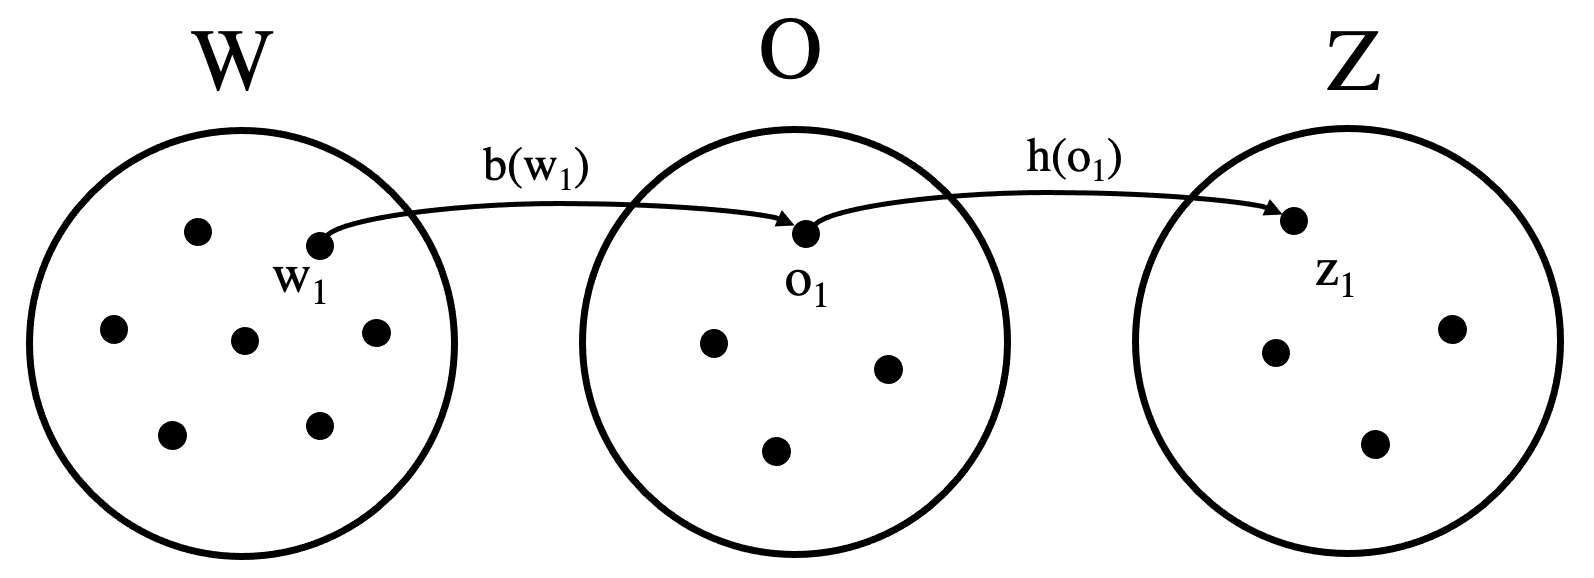
\includegraphics[scale = 0.35]{3ReproducingSBDRL/Old/Images/W_to_O_to_Z_mapping.png}
    \caption{The composite mapping from the set $W$ of world states to the set $Z$ of state representations via the set $O$ of observations.}
    \label{fig:observation-maps}
\end{figure}

\paragraph{Groups and symmetries}
\begin{definition}[Group]
    A group $G$ is a set with a binary operation $G \times G \to G$, $(g, g') \mapsto g \circ g'$ called the \textit{composition} of group elements that satisfies the following properties:
\begin{enumerate}
    \item \textit{Closure.}
    $g \circ g'$ is defined for all $g, g' \in G$.
    \item \textit{Associative.}
    $(g \circ g') \circ g'' = g \circ (g' \circ g'')$ for all $g, g', g'' \in G$.
    \item \textit{Identity.}
    There exists a unique identity element $1 \in G$ such that $1 \circ g = g \circ 1 = g$ for all $g \in G$.
    \item \textit{Inverse.}
    For any $g \in G$, there exists $g^{-1} \in G$ such that $g \circ g^{-1} = g^{-1} \circ g = 1$.
\end{enumerate}
\end{definition}

Applying symmetries to objects is mathematically defined as a \textit{group action}.

\begin{definition}[Group action]
    Given a group $G$ and a set $X$, a group action of $G$ on $X$ is a map $G \times X \to X$, $(g,x) \mapsto g * x$ that satisfies the following properties:
\begin{enumerate}
    \item \textit{Compatibility with composition.}
    The composition of group elements and the group action are compatible: $g' \circ (g * x) = (g' \circ g) * x$ for $g,g' \in G$ and $x \in X$.
    \item \textit{Identity.}
    The group identity $1 \in G$ leaves the elements of $X$ unchanged: $1 * x = x$ for all $x \in X$.
\end{enumerate}
\end{definition}



Another important property of groups is commutation.
Two elements of a group \textit{commute} if the order they are composed does not matter: $g \circ g' = g' \circ g$.
If all elements in a group commute with each other then the group is called \textit{commutative}.
Subgroups of a group might commute with each other.

\paragraph{\sout{Symmetry-based representations}}
\sout{
The set $W$ of world states has a set of symmetries that are described by the group $G$.
This group $G$ acts on the set $W$ of world states via a group action $\cdot_{W}: G \times W \to W$.
For the agent's representations $z_i \in Z$ to be symmetry-based representations, a corresponding group action $\cdot_{Z}: G \times Z \to Z$ must be found so that the symmetries of the agent's representations reflect the symmetries of the world states.
The mathematical condition for this is that, for all $w \in W$ and all $g \in G$, applying the action $g \cdot_W$ to $w$ and then applying the mapping $f$ gives the same result as first applying the mapping $f$ to $w$ to give $f(w)$ and then applying the action $g \cdot_Z$ to $f(w)$.
Mathematically, this is $f(g \cdot_W w) = g \cdot_Z f(w)$.
If this condition is satisfied, then $f$ is called a \textit{group-equivariant map}.
}

\paragraph{\sout{Symmetry-based disentangled representations}}
\sout{
To go from symmetry-based representations to symmetry-based disentangled representations, suppose the group of symmetries $G$ of the set $W$ of world states decomposes as a direct product $G = G_1 \times \hdots \times G_i \times \hdots \times G_n$.
The group action $\cdot_Z : G \times Z \to Z$ and the set $Z$ are disentangled with respect to the decomposition of $G$, if there is a decomposition $Z = Z_1 \times \hdots \times Z_i \times \hdots \times Z_n$ and actions $\cdot_{Z_i}: G_i \times Z_i \to Z_i, i \in \{1, \hdots, n\}$ such that $(g_{G_1}, g_{G_2}) \cdot_Z (z_{Z_1}, z_{Z_2}) = (g_{G_1} \cdot_{Z_1} z_{Z_1}, g_{G_2} \cdot_{Z_2} z_{Z_2})$, where $g_{G_i} \in G_i$ and $z_{Z_i} \in Z_i$.
In other words, each subspace $Z_i$ is invariant to the action of all the $G_{j \neq i}$ and only affected by $G_i$.
}

\paragraph{\sout{Summary}}
\sout{
The representations in $Z$ are symmetry-based disentangled with respect to the decomposition $G = G_1 \times \hdots \times G_i \times \hdots \times G_n$, where each $G_i$ acts on a disjoint part of $Z$, if:
}
\begin{enumerate}
    \item \sout{There exists a group action $\cdot_{W}: G \times W \to W$ and a corresponding group action $\cdot_{Z}: G \times Z \to Z$;}
    \item \sout{The map $f : W \to Z$ is group-equivariant between the group actions on $W$ and $Z$: $g \cdot_{Z} f(w) = f(g \cdot_{W} w)$. In other words, the diagram}
    % https://q.uiver.app/#q=WzAsNCxbMCwwLCJ3Il0sWzIsMCwiZyBcXGNkb3Rfe1d9IHciXSxbMCwyLCJmKHcpIl0sWzIsMiwiZyBcXGNkb3Rfe1p9IGYodykgPSBmKGcgXFxjZG90X3tXfSB3KSJdLFswLDEsImcgXFxjZG90X3tXfSJdLFswLDIsImYiLDJdLFsxLDMsImYiLDJdLFsyLDMsImcgXFxjZG90X3tafSJdXQ==
\[\begin{tikzcd}
	w && {g \cdot_{W} w} \\
	\\
	{f(w)} && {g \cdot_{Z} f(w) = f(g \cdot_{W} w)}
	\arrow["{g \cdot_{W}}", from=1-1, to=1-3]
	\arrow["f"', from=1-1, to=3-1]
	\arrow["f"', from=1-3, to=3-3]
	\arrow["{g \cdot_{Z}}", from=3-1, to=3-3]
\end{tikzcd}\]

    \sout{commutes.}

    \item \sout{There exists a decomposition of the representation $Z = Z_1 \times \hdots \times Z_n$ such that each subspace $Z_i$ is unaffected by the action for all $G_{j \neq i}$ and is only affected by $G_i$.}
\end{enumerate}


\paragraph{Limitations of SBDRL}
Both \cite{Higgins2018} and \cite{caselles2019symmetry} suggest that these group actions can be used to describe some types of real-world actions.
However, it is important to note that they do not believe that all actions can be described by their formalism: \textit{``It is important to mention that not all actions are symmetries, for instance, the action of eating a collectible item in the environment is not part of any group of symmetries of the environment because it might be irreversible.''}
\whendraft{
\textbf{Need to cite pg4 of caselles2019symmetry:}
% \cite[page 4]{caselles2019symmetry}.
}

